\subsection{Comparison to Commercial VNAs}

Testing of the VNA consists of comparing measurements against commercial devices, and seeing how well correlated the results are. Comparisons were primarily done against an Agilent ENA Network Analyser, however due to the ENA only having a N-Type calibration kit whilst the DUTs had SMA connectors, it was unable to be used for phase measurements. For the phase measurements, a NanoVNA was utilised, which is a low cost VNA capable of functioning up to 900 MHz. Although the NanoVNA is a low cost device purchased from Ebay, it has been shown to function well enough against commercial offerings (Keysight Fieldfox) \cite{nanoVNA} that it is sufficient for use as a comparison. 

Figure \ref{fig:compare_900_s11} shows the measurement of a lumped element 900 MHz low pass filter. As can be seen, the VNA tracks fairly well, with discrepancies between the traces maximised when the magnitude ratio decreases below -20 dB, or when there is a rapid change in frequency response. The changes at lower power levels can be explained by the dynamic range of the instrument when measuring reflected power being around -25 dB.

The dynamic range of the instrument has two primary contributors: directivity of the coupler and dynamic range of the AD8302 gain and phase detector. The Mini Circuits ADC-15-4+ directional coupler utilised has between 24 and 33 dB of directivity over the frequency range of operation, which means that it is unable to differentiate any signals travelling in the forward or reverse direction below this magnitude, and as such can not identity reflected signals smaller than its dynamic range. The dynamic range of the detector is another factor, as the AD8302 can only measure differences in gain within a $\pm$30 dB range between the two RF inputs. 

As such, S\textsubscript{11} measurements will have a minimum guaranteed dynamic range of 24 dB, ranging up to 30 dB at frequencies where the dynamic range of the AD8302 becomes a limiting factor. For S\textsubscript{21} measurements which are terminated directly into the AD8302, there are no directional couplers to limit directivity and as such there is 30 dB of dynamic range. This difference in dynamic range can be seen by comparing Figures \ref{fig:compare_900_s11} and \ref{fig:compare_lfcn_s21}, where it can be seen that the dynamic range of the S\textsubscript{21} measurement in Figure \ref{fig:compare_lfcn_s21} is around 33 dB, whereas the S\textsubscript{11} measurements in Figure \ref{fig:compare_900_s11} has a maximum of approximately 27 dB. Due to corrections resulting from calibration the plotted numbers are slightly greater than theoretical, and this will be discussed later. 

With respect to the VNA not measuring the changing frequency response around 930 MHz, it is not related to the frequency response changing too quickly to be measured as there is ample time for the device to sample, however it may be a result of decreased dynamic range caused by harmonics passing from the LO to the detector, which will be discussed later with reference to Figure \ref{fig:power_unlevel}. 
\begin{figure}[H]
	\centering
	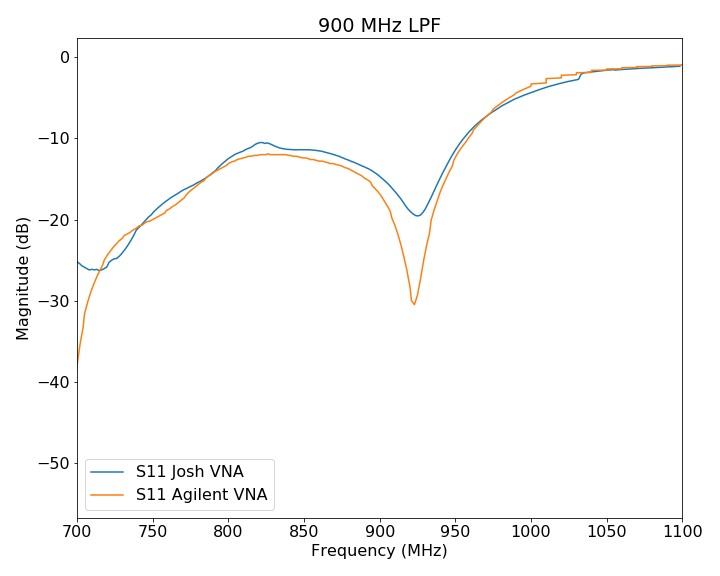
\includegraphics[width=0.8\linewidth]{900_MHz_LPF_s11.png}
	\caption{S\textsubscript{11} comparison of a 900 MHz low pass filter}
	\label{fig:compare_900_s11}
\end{figure}

Figure \ref{fig:compare_900_s21} shows an S\textsubscript{21} measurement of the same lumped element filter. There is some ripple in the passband from the VNA, along with it measuring above unity between 700 MHz and 800 MHz. This is related to the issue with LO flatness and harmonics, and will be discussed below with reference to Figure \ref{fig:power_unlevel}. The offset in frequency to the right of the commercial VNA can also be seen in Figure \ref{fig:compare_lfcn_s21}, and is most likely caused by a bug in the phase correction step, where the signal is low pass filtered which results in a lower number of elements in the set which shifts the frequency response to the left (down in frequency), and then is moved back to the correct frequencies. Given that this issue is found in both S\textsubscript{21} measurements and not S\textsubscript{11} measurements, where the phase correction algorithm does not have to deal with as many corrections due to the decreased electrical length when measuring S\textsubscript{11} directly against port 1 of the VNA, instead of through a length of coax as is required with S\textsubscript{21} measurements, it can most likely be resolved, however unfortunately there is insufficient time to explore this further. 

\begin{figure}[H]
	\centering
	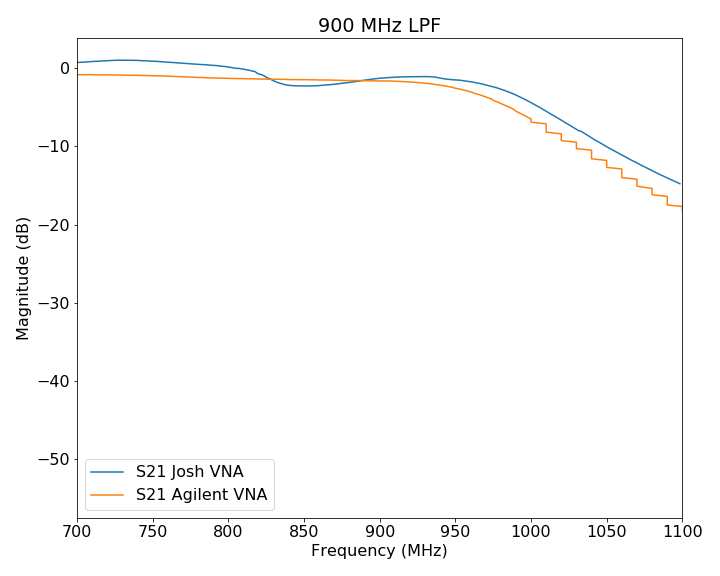
\includegraphics[width=0.8\linewidth]{900_MHz_LPF_s21.png}
	\caption{S\textsubscript{21} comparison of a 900 MHz low pass filter}
	\label{fig:compare_900_s21}
\end{figure}

Figure \ref{fig:power_unlevel} shows the power flatness from the transmit chain, and was determined by measuring S21 with both ports of the VNA terminated into 50$\Omega$ loads. Whilst this measurement would typically referred to as isolation between port 1 and 2, due to the AD8302 measuring the difference between the LO and port 2, it shows both the isolation between ports, along with the flatness of the LO in a single measurement which cannot be separated. Given both ports are terminated and the frequencies are fairly low which will result in reduced coupling between ports, it can be assumed that all of the changes in magnitude are a direct result of the power from the LO changing as a function of frequency. 

The rapid changes in power as a function of frequency are a combination of the large number of harmonics in the MAX2871 output due to it utilising a divided down output below 3 GHz, and as such the output waveform is a square wave which has numerous harmonics at integer multiples of the fundamental, along with poor filter choices to remove the harmonics, as described in \S \ref{subsubsec:lo filtering}. At the time of design it was not known that the output of the MAX2871 (and other low cost, single chip PLLs) were divided down to increase their frequency range, as it was not specified in the documentation and there was no prior experience with the IC. This resulted in the assumption that significant filtering would not be required, as any harmonics would be a significant number of dB down from the fundamental and would not impact the measurement significantly. During bring-up of the transmit chain it was connected to a spectrum analyser and the large number of harmonics was noticed, as previously measurements were done with a low bandwidth (50 MHz) oscilloscope which was unable to capture past the first harmonic and as such appeared to be less of an issue. It should be noted that the measurements done on the oscilloscope were made during bring-up of the MAX2871 and associated firmware, and were aimed to capture if there was an output and if so what was the frequency as this was a major challenge during development, and was not aimed to assess the signal quality of the output waveform due to the lack of bandwidth which would limit the representation of the signal. 

\begin{figure}[H]
	\centering
	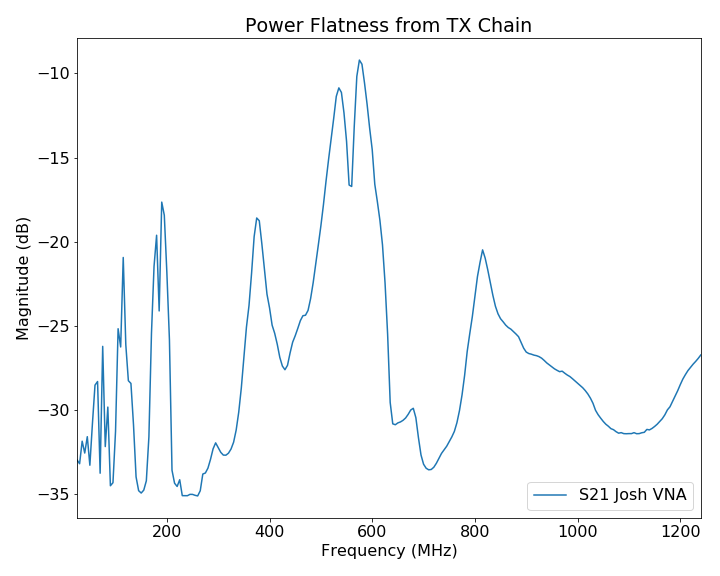
\includegraphics[width=0.8\linewidth]{power_unlevel.png}
	\caption{Power flatness from TX chain, measurements shown S\textsubscript{21} with both ports terminated into 50$\Omega$}
	\label{fig:power_unlevel}
\end{figure}

This behaviour shows itself in two main effects: ripple in the magnitude response and decreased dynamic range. The issue with ripple is most easily seen in Figure \ref{fig:compare_lfcn_s21}, where there is a noticeable peak at 550 - 600 MHz, which corresponds with the spike in power shown in Figure \ref{fig:power_unlevel}. With respect to dynamic range, it can be seen that when there is an increased reference waveform such as at 900 - 950 MHz, the measured response at that frequency (such as shown in Figure \ref{fig:compare_900_s11}) is not as low as should be. This occurs for the same reason as above, as the increased reference power increases the measured result, which presents itself as an increased noise floor.  

There are two primary methods which could be used to resolve this issue: changing the number and cut-off frequency of the filters, and changing to a superheterodyne architecture. Increasing the number of filters would allow for sufficient attenuation of harmonics across the frequency band, however going above four filters is impracticable due to the availability of switches with more than four ports, along with the significant amount of space filter banks take up. To improve performance whilst only utilising four filters, the frequency range of the VNA would need to be reduced, which is undesirable. In saying this, changing the filters would be the easiest option as it could be done to the currently assembled board with some flux and a hot air gun. 

Altering the architecture of the VNA to a superheterodyne device where the inputs to the AD8302 are downconverted to a fixed frequency would also resolve this issue, as a single filter could be used at the inputs of the receiver to filter out any unwanted frequencies as they would be downconverted to outside the bandwidth of the filter. Whilst this method would add an additional MAX2871 and two mixers to the BOM, filtering on the transmit chain could be removed which would save cost, along with allowing the VNA to function up to 6 GHz if the directional couplers are replaced during redesign of the PCB. This would however be a significant investment from a time and resource perspective, and a redesign of this nature should only be attempted if all other aspects of the VNA are shown to be working nominally to reduce the risk of having the redesign not function as desired. 

Figure \ref{fig:compare_lfcn_s21} shows the insertion loss of a 400 MHz filter from Mini Circuits (LFCN-400+) which due to it's internal construction as a multiple order device has a sharp roll off and significant (> 50 dB) attenuation in the stop band. The VNA exhibits frequency shifting and ripple in the passband as discussed above, and in addition does not have the dynamic range below 30 dB to show the full response of the filter. It does however roughly track the frequency response of the device even though it is unable to measure below 30 dB, and as such may be used for indicative measurements if a VNA or other test gear cannot be sourced to determine the exact frequency response. 
\begin{figure}[H]
	\centering
	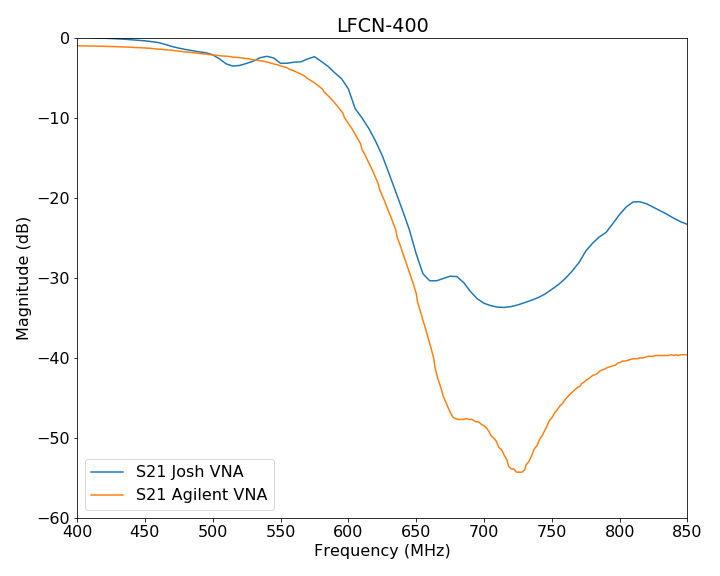
\includegraphics[width=0.8\linewidth]{LFCN-400-s21.png}
	\caption{S\textsubscript{21} comparison of a LFCN-400+ low pass filter}
	\label{fig:compare_lfcn_s21}
\end{figure}

Looking at a Smith Chart representation of the LFCN-400+ filter in Figure \ref{fig:compare_lfcn_smith}, it can be seen that there are issues with the phase measurements. Whilst the trace generally follows the expected path, it appears to have incorrect phase values in the center of the chart, where it's location relative to 50$\Omega$ is flipped, along with the path it takes until halfway between the center and edge of the chart. The large spike at 11 o'clock is a result of the dip at 500 - 550 MHz in Figure \ref{fig:compare_lfcn_s21} and is a separate issue to the phase measurement. 

This behaviour has been seen on numerous measurements, and typically occurs whenever there is a rapid change in frequency response, such as the roll off of a filter, or resonant frequency of an antenna. Whilst the cause of this is uncertain, the strange phase response can be seen from the raw AD8302 samples, and is only slightly improved when correction is applied from the calibration process. This is a problem where utilising an evaluation board with control over the amplitude and phase difference of the two input signals would be ideal, as the causal reasoning behind the undesirable output could be found, or it may not occur and then issues in other areas of the board could be investigated. In an attempt to resolve this, an AD8302 development board along with dual signal generators were acquired to allow investigation, however due to a lack of time this was unable to be attempted and as such the cause remains unknown. 

\begin{figure}[H]
	\centering
	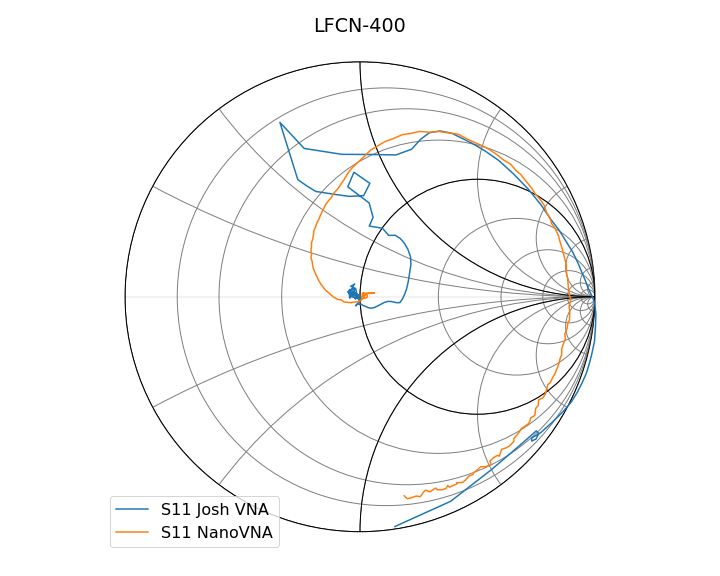
\includegraphics[width=0.8\linewidth]{LFCN-400-smith.png}
	\caption{S\textsubscript{11} comparison of a LFCN-400+ low pass filter}
	\label{fig:compare_lfcn_smith}
\end{figure}

\subsection{Calibration Efficacy}
One of the key performance metrics of a VNA is how well it can be calibrated, as this sets the measurement quality for any DUTs being measured. Figure \ref{fig:cal_sucks} shows a comparison between the load calibration standard, and the calibrated and uncalibrated measurements from the VNA. The calibration does a fairly good job at correcting the measurement so that it represents the load standard, however there are a few issues resulting from power flatness and dynamic range which cause issues with the calibration. 

Looking at the LF to 250 MHz range of the S\textsubscript{11} plot, it can be seen that the dynamic range of the AD8302 is unable to follow the > 60 dB of the calibration standard, and as a result the calibrated response is jumping all over the place in an attempt to compensate for the difference. This results in issues with the compensated phase values, which rapidly jump between +100$^\circ$ to -100$^\circ$, which is undesirable. Unfortunately this is an inherent issue with the architecture of the system and as such cannot be resolved through a hardware revision, however attempting to calibrate it against a load standard which has been altered to only have approximately a -25 dB match at low frequencies may possibly resolve this issue, as the calibration will no longer have to try adding dynamic range to the measured values. 

\begin{figure}[H]
	\centering
	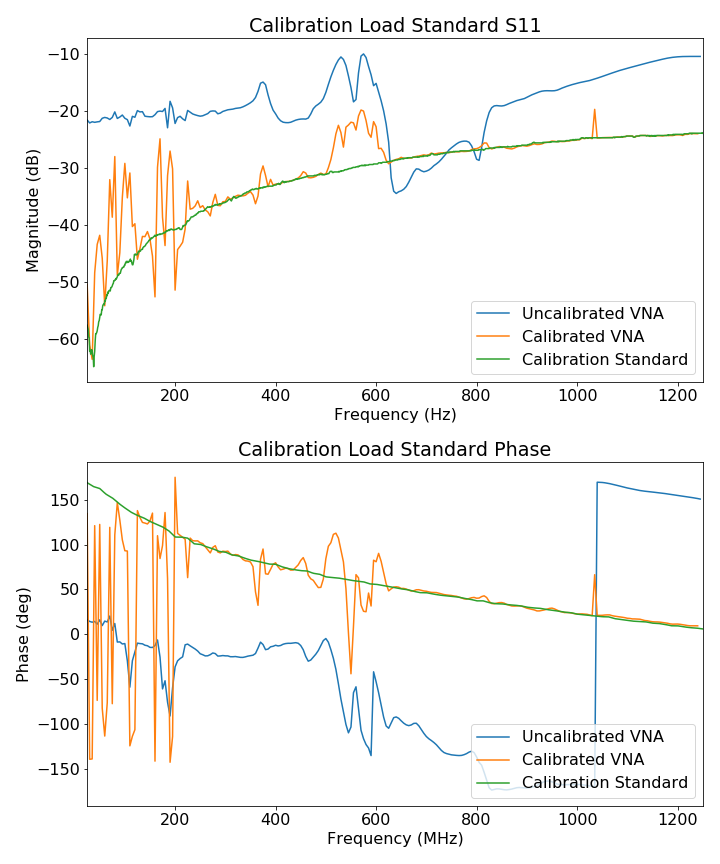
\includegraphics[width=0.8\linewidth]{load_cal_issues.png}
	\caption{S\textsubscript{11} and Phase measurements for a calibration load standard, with correction disabled and enabled.}
	\label{fig:cal_sucks}
\end{figure}

Another issue identified is the calibration not being able to compensate for large changes in power level, seen in the 500 - 600 MHz peak seen after correction. This is likely due to the twelve term calibration not accounting for LO unevenness to such a degree, and as such can not generate compensation terms to correct for the large gain in power, along with decreased dynamic range at the receiver due to the reference level increasing significantly. 

With this said, excluding the spike in magnitude at 1050 MHz due to the wrapping of phase from -180$^\circ$ to +180$^\circ$, the VNA tracks the calibration standard quite well between 600 and 1250 MHz, which suggests that if the prior two issues are rectified it may well function as expected over the whole frequency range. 

\subsection{Conclusion and Future Work}
Through research into how vector network analysers function, architecture and component selections to optimise performance of the device whilst meeting constraints, design and assembly of a RF PCBA, along with firmware and software development, a low cost VNA was designed, assembled, and tested. Due to issues with architecture and component selection there were numerous issues with the VNA which resulted in it's performance not being sufficient for the desired use cases, however the issues were identified and potential fixes suggested, which if implemented in a new revision may result in a VNA which meets the design goals. 

The key issues identified which should be looked into if future work is to be done are outlined below: 
\begin{itemize}
	\item \textbf{LO Power Flatness} needs to be resolved, with possible solutions including altering filter choices to ensure harmonics are sufficiently attenuated, altering the architecture to add a superheterodyne stage to the receiver which would result in unwanted frequencies being downconverted to outside the filter passband, or potentially selecting a new LO which has a much cleaner output spectrum.
	\item \textbf{Rectify Issues with Phase Measurements at Magnitude Transitions} is key to ensuring that the phase measurement is correct when there is a change in magnitude response, such as at a filter cut-off frequency, or at an antennas resonant frequency. 
	\item \textbf{Calibration Improvements} including resolving issues when the dynamic range of the AD8302 is insufficient to measure the DUT, along with resolving the spike in magnitude and phase when the phase wraps around on the uncorrected measurement. 
\end{itemize}
Furthermore the user experience could be improved through the addition of a graphical user interface, along with extensive documentation on how to use and modify the device, however this should only be implemented if the issues above are able to be corrected and a VNA which has sufficient accuracy is able to be implemented. 

With this said, even though the function of the VNA was not as desired there was a significant amount of insight and knowledge gained in the areas of RF design, PCB layout and assembly, along with firmware and software development which has resulted in increased technical and non technical skills which has been invaluable for professional development. 